%%%%%%%%%%%%%%%%%%%%%%%%%%%%%%%%%%%%%%%%%%%%%%%%%%%%%%%%%%%%%%%%%%%%%%%%%%%%%%%%
%2345678901234567890123456789012345678901234567890123456789012345678901234567890
%        1         2         3         4         5         6         7         8

\documentclass[letterpaper, 10 pt, conference]{ieeeconf}  % Comment this line out if you need a4paper

%\documentclass[a4paper, 10pt, conference]{ieeeconf}      % Use this line for a4 paper

\IEEEoverridecommandlockouts                              % This command is only needed if
                                                          % you want to use the \thanks command

\overrideIEEEmargins                                      % Needed to meet printer requirements.

% See the \addtolength command later in the file to balance the column lengths
% on the last page of the document

% The following packages can be found on http:\\www.ctan.org
\usepackage{graphics} % for pdf, bitmapped graphics files
\usepackage{epsfig} % for postscript graphics files
%\usepackage{mathptmx} % assumes new font selection scheme installed
%\usepackage{times} % assumes new font selection scheme installed
\usepackage{amsmath} % assumes amsmath package installed
\usepackage{amssymb}  % assumes amsmath package installed
\usepackage{url}
\usepackage{subfigure}
% Rafael
\usepackage{xspace}
\usepackage{pgfplots}
\usepackage{graphicx}
\usepackage{epstopdf}
\usepackage{cite}


% axded by Rafael
%%%%%%%%%%%%%%%%%%%%%%%%%%%%%%%%%%%%%%%%%%%%%%%%%%%%%%%%%%%%%%%
\def\marhes{{\sc Marhes}\xspace}
\def\octor{{OctoRoACH}\xspace}
\def\octors{{OctoRoACHes}\xspace}
\def\turtle{{TurtleBot}\xspace}
\def\turtles{{TurtleBots}\xspace}
\newcommand{\ie}{{\it i.e.},\xspace}
\newcommand{\eg}{{\it e.g.},\xspace}
\newcommand{\cf}{{\it c.f.},\xspace}
\newcommand{\el}{{\it et al.},\xspace}
\newcommand{\etc}{\text{etc.}}

\providecommand{\norm}[1]{\left\lVert#1\right\rVert}

%% Math defs
% The set of reals, integers, etc.
\renewcommand{\Re}{\mathbb{R}}
\newcommand{\Ze}{\mathbb {Z}}
\newcommand{\Pe}{\mathbb {P}}
\newcommand{\I}{\mathcal{I}}

\newtheorem{definition}{Definition}
%%%%%%%%%%%%%%%%%%%%%%%%%%%%%%%%%%%%%%%%%%%%%%%%%%%%%%%%%%%%%%

\title{\LARGE \bf
Homework 1 
}

\author{Luis A. Valbuena Reyes% <-this % stops a speeeeace
%\thanks{*This work was not supported by the MAST project.}% <-this % stops a space
\thanks{Luis Valbuena is with the Department of Electrical and Computer Engineering,
        University of New Mexico, Albuquerque, NM, 87131-0001, {\tt\small \{lavalbuenar@unm.edu}}%
}

\begin{document}

\newtheorem{theoremMyThesis}{Theorem}
\newtheorem{corollary}{Corollary}
\newtheorem{problemStatement}{Problem Statement}

\maketitle
\thispagestyle{empty}
\pagestyle{empty}


%%%%%%%%%%%%%%%%%%%%%%%%%%%%%%%%%%%%%%%%%%%%%%%%%%%%%%%%%%%%%%%%%%%%%%%%%%%%%%%%
\begin{abstract}

In this document, we present the solution for homework 1. We are required to use to function \emph{svmtrain} and \emph{svmpredict}
from the package LIBSVM. Trying to follow the guidelines for writing papers, we develop each the requirements of the assignment on Sections \ref{sec:theory}, \ref{sec:experiments}, and \ref{sec:conclusion}.
\end{abstract}


%%%%%%%%%%%%%%%%%%%%%%%%%%%%%%%%%%%%%%%%%%%%%%%%%%%%%%%%%%%%%%%%%%%%%%%%%%%%%%%%

\section{INTRODUCTION}
\label{sec:Intro}

This assignment was about how the support vector machine technique behave under different scenarios.

%%%%%%%%%%%%%%%%%%%%%%%%%%%%%%%%%%%%%%%%%%%%%%%%%%%%%%%%%%%%%%%%%%%%%%%%%%%%%%%%

\section{Theory}
\label{sec:theory}

\subsection{Construction of a classifier with the model parameters}
\label{sec:TheoryConstructionClassifierModelParameters}

Taking care of conducting matrix operations with compatible dimensions\footnote{The dimensions of the quantities 
in the code are not compatible with the matrix multiplications presented on some of the slides}, we construct the 
simplest machine:

\begin{equation*}
    \hat{\mathbf{y}} = \mathbf{Xw},
\end{equation*}
where it is suggested to calculate $\mathbf{w}$ from the parameters $\alpha_{i}$ and the data, $\mathbf{X}$. That is:
                          
\begin{equation*}
   \mathbf{w} = \mathbf{X}^{T} \mathbf{\alpha} \quad \text{with } \mathbf{\alpha} = (\mathbf{XX}^{T})^{-1}\mathbf{y},
\end{equation*}
where $y$ are the labels associated with the samples in $X$. The matrix $(XX^{T})^{-1}$ is problematic because it is ill 
conditioned. Then, using the reduced single value decomposition $X = \mathbf{U}\mathbf{\Sigma} \mathbf{V}^{T}$:

\begin{equation*}
\begin{aligned}
    \alpha &= (\mathbf{XX}^{T})^{-1}\mathbf{y}, \\
                 &= (\mathbf{U} \mathbf{\Sigma} \mathbf{V}^{T}(\mathbf{U}\mathbf{\Sigma} \mathbf{V}^{T})^{T})^{-1}\mathbf{y},\\
                 &= (\mathbf{U} \mathbf{\Sigma} \mathbf{V}^{T} \mathbf{V} \mathbf{\Sigma}^{T} \mathbf{U}^{T})^{-1}\mathbf{y},\\
                 &= (\mathbf{U} \mathbf{\Sigma}^{2} \mathbf{U}^{T})^{-1}\mathbf{y},\\
                 &= \mathbf{U}\mathbf{\Sigma}^{-2} \mathbf{U}^{T} \mathbf{y}
\end{aligned}
\end{equation*}
where matrices $ \mathbf{U}$ and $ \mathbf{V}$ are unitary. The machine is then:
\begin{equation*}
    \hat{ \mathbf{y}} = \mathbf{ Xw}=  \mathbf{X X}^{T} \mathbf{U \Sigma}^{-2}  \mathbf{U}^{T}  \mathbf{y}.
\end{equation*}

Then, for a single sample $x_{i}$, we have $ \hat{ \mathbf{y}}_{i} = x_{i}\mathbf{w}$. The results are presented on Section  \ref{sec:ExperimentConstructionClassifierModelParameters}.

On the other hand, we have a tool called support vector machines, which finds a balance between complexity and regularization. On the minimization of the mean-squared error, we are increasing the complexity of the solution, which can lead to an over-fitting of the learner: the machine will be learning the noise of the data along. Then given a linear classifier of the form $f(\mathbf{X}) = \mathbf{w}^{T}\mathbf{X} + b$ we minimize the error measure and also the magnitude of $ \mathbf{w}$, which in turn minimizes the complexity. The algorithm is minimize

\begin{equation*}
 \| \mathbf{w} \| + C \sum_{i} \xi_{i}, \text{ subject to } y_{i}(\mathbf{w}^{T}x_{i} + b ) \geq 1 - \xi_{i}.
\end{equation*}

The region between the planes $y_{i}(\mathbf{w}^{T}x_{i} + b ) \geq 1 $ is called the margin and the only data that takes place in the support vector algorithm are
the samples that are inside the margin and the samples that are completely misclassified with respect to the classifier, see Fig.~\ref{fig:SupportVectorImage}

\begin{figure}[thpb]
      \centering
      \framebox{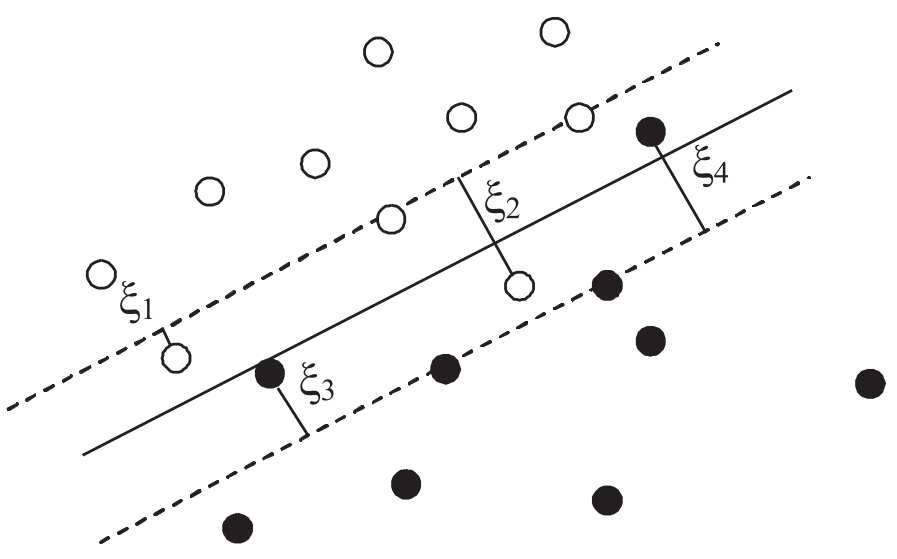
\includegraphics[scale=.25]{SolutionMaterial/SupportVectorImage.png}}
      \caption{Support Vector machine schematics. Taken from the class notes. }
      \label{fig:SupportVectorImage}
\end{figure}


\subsection{Graphical representation of an SVM}
\label{sec:TheoryGraphicalRepresentationSVM}

The function \emph{svmtrain} has the option of displaying the data with the separating line and the support vectors. To draw 
the two margin lines, we created a meshgrid, evaluated the support vector machine given by @svmtrain@ with the margin 
offset $\pm1$ and plot the contour where $f(X) = 0$. The results are presented on Section \ref{sec:ExperimentGraphicalRepresentationSVM}.

 \subsection{Estimating Structural Risk}
 \label{sec:TheoryEstimatingStructuralRisk}
 
 In \cite{Burges1998}, for a group of $l$ predictors, the empirical risk (error) is given as:
 
 \begin{equation}
  R_{emp}(\alpha) = \frac{1}{2l} \sum_{i=1}^{l} \mid y_{i} - f(\mathbf{x}_{i},\alpha) \mid,
  \label{eq:Error}
 \end{equation}
 
 where $\mathbf{x}_{i}$ and $y_{i}$ are the data from the training set. The instructor advised  to use the same expression using $\mathbf{x}_{i}$ and $y_{i}$ from
 the test set to calculate the actual risk. The structural risk is the difference between the actual risk and empirical risk.  The results are presented on Section  \ref{sec:ExperimentEstimatingStructuralRisk}.

\subsection{SVM for Regression}
\label{sec:TheorySVMRegression}

This experiment requires us to simulate the linear process
\begin{equation*}
\begin{aligned}
   y[n] &= 0.03y[n-1] - 0.01y[n-2] \\ &+ 3x[n] - 0.5x[n-1] + 0.2x[n-2],
\end{aligned}
\end{equation*}
where $x[n]$, $x[n-1]$ and $x[n-2]$ are the inputs. Preliminarily, it was assumed that $x[n]$, $x[n-1]$ and $x[n-2]$
were the attributes and $y[n]$ the label, but note that $y[n-1]$ and $y[n-2]$ also take part on  $y[n]$. Therefore, it
is required to precompute the kernel used by the support vector machine algorithm to specify  what are the labels 
and the attributes. The input is $N(0,1)$ and the signal $y[n]$ is disturbed by additive noise of the form $e[n] ~ N(0, 0.01)$. 
The idea of this theoretical example is that we only have $x[n]$ and  $y[n]+e[n]$ and we reconstruct $y[n]$. Let $o[n] = y[n]+e[n]$. 
Based on the advice given by the instructor, the new attributes and labels are of the form:

\begin{equation*}
 Z_{i} = \begin{bmatrix} x[i-2] \\ x[i-1] \\ x[i]\\ o[i-2] \\ o[i-1] \end{bmatrix},\quad Y_{i} = o[i],
\end{equation*}
for $i \geq 2$. Then $\mathbf{Z} = [  Z_{2} \quad Z_{3} \quad \hdots \quad  Z_{N}]$ and $\mathbf{Y} = [  o_{2} \quad o_{3} \quad \hdots \quad  o_{N}]^{T}$.
The precomputed kernel has the form $\mathbf{K} = \gamma \mathbf{I} + \mathbf{Z}^{T}\mathbf{Z}$. 

The results are presented on Section  \ref{sec:ExperimentSVMRegression}. The RMS error is calculated between the output $y[n]$ and the estimated $\hat{o}[n]$ signal given by the calculated support vector machine.
%%%%%%%%%%%%%%%%%%%%%%%%%%%%%%%%%%%%%%%%%%%%%%%%%%%%%%%%%%%%%%%%%%%%%%%%%%%%%%%%

\section{Experiments}
\label{sec:experiments}

This is the output of the command  @svmtrain@ given on the sample code, see Fig.~\ref{fig:NormalExecution}

%\begin{figure}[thpb]
%      \centering
%      \framebox{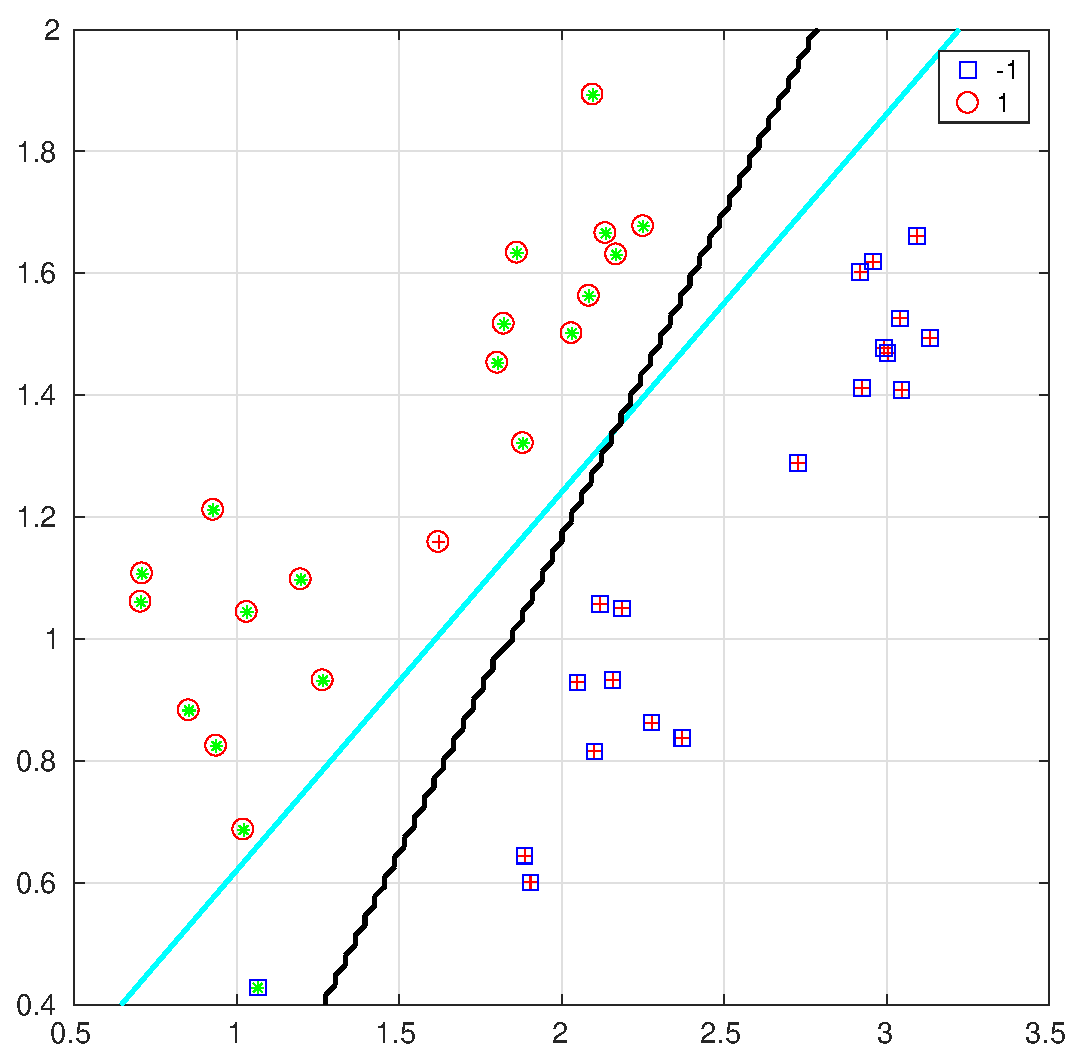
\includegraphics[scale=.35]{SolutionMaterial/Comparizon.eps}}
%      \cprotect  \caption{Output of  @svmtrain@. }
%      \label{fig:NormalExecutionsvmtrain}
%\end{figure}

\subsection{Construction of a classifier with the model parameters}
\label{sec:ExperimentConstructionClassifierModelParameters}

The comparizon requested can be appretiated on Fig.~\ref{fig:NormalExecution} and Fig.~\ref{fig:Comparizon}. 


\begin{figure}[ht!]
 \begin{center}
  	\subfigure[\label{fig:NormalExecution}]{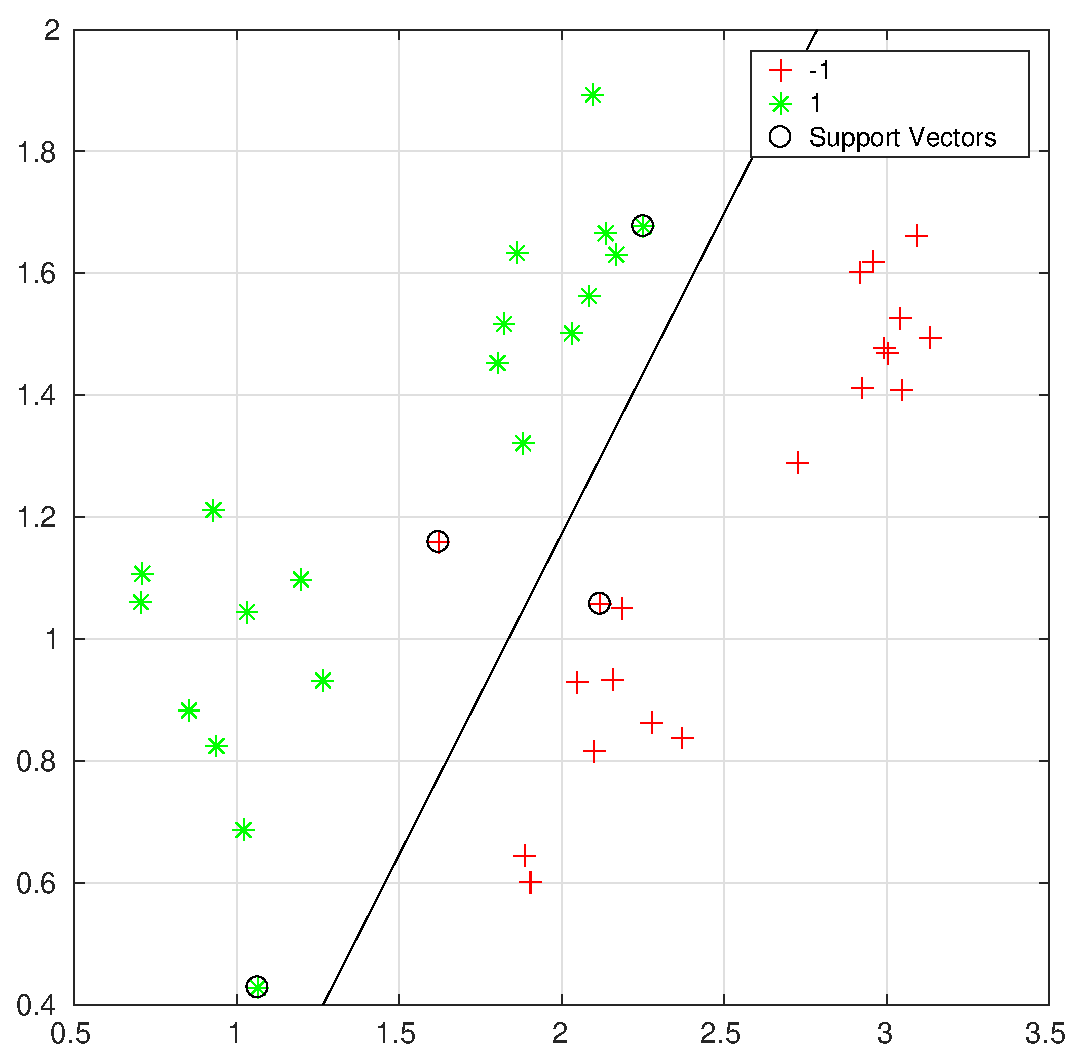
\includegraphics[width=0.42\textwidth]{SolutionMaterial/NormalExecution.eps}}
 	\subfigure[\label{fig:Comparizon}]{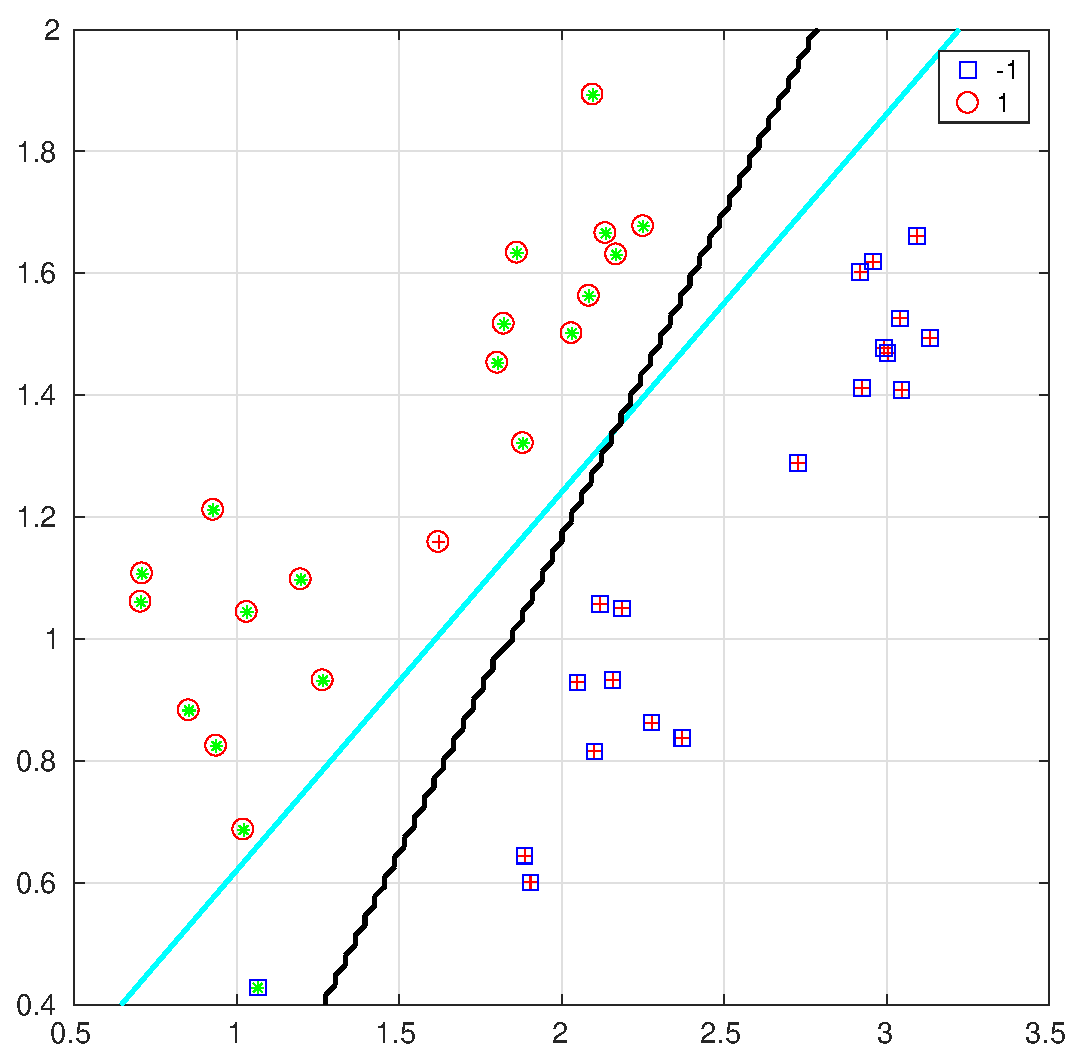
\includegraphics[width=0.42\textwidth]{SolutionMaterial/Comparizon.eps}}
         \caption{Output of \emph{svmtrain}. (a), Normal Execution. (b) The constructed machine.}
 \end{center}
\end{figure}

This time, the samples that the constructed machine classifies as $1$  are assigned a red circle marker, while the 
others are assigned a blue square marker. The stepped black\footnote{This line is a contour line for which the classifier is zero. 
The step feature of the line is due to the mesh grid used.} line on  Fig.~\ref{fig:Comparizon} is the black line on Fig.~\ref{fig:NormalExecution}, 
and the cyan line is a contour line of the plane perpendicular to $ \mathbf{w}$ as $x_{i}\mathbf{w}=0$. Note that these planes 
are not parallel. Also note that for this particular experiment,  the sample in the region $1 \leq x \leq1.5$ and $0.4 \leq y \leq 0.6$ 
is misclassified by the constructed machine.

\subsection{Graphical representation of an SVM}
\label{sec:ExperimentGraphicalRepresentationSVM}

We chose $\sigma = \{0.05, 1, 1.4\}$, the plots of the separating line, the two
margin lines and the support vectors are presented in Fig.~\ref{fig:svm_sigma_5}, Fig.~\ref{fig:svm_sigma_100}, and  
Fig.~\ref{fig:svm_sigma_140}.

\begin{figure}[ht!]
 \begin{center}
  	\subfigure[\label{fig:svm_sigma_5}]{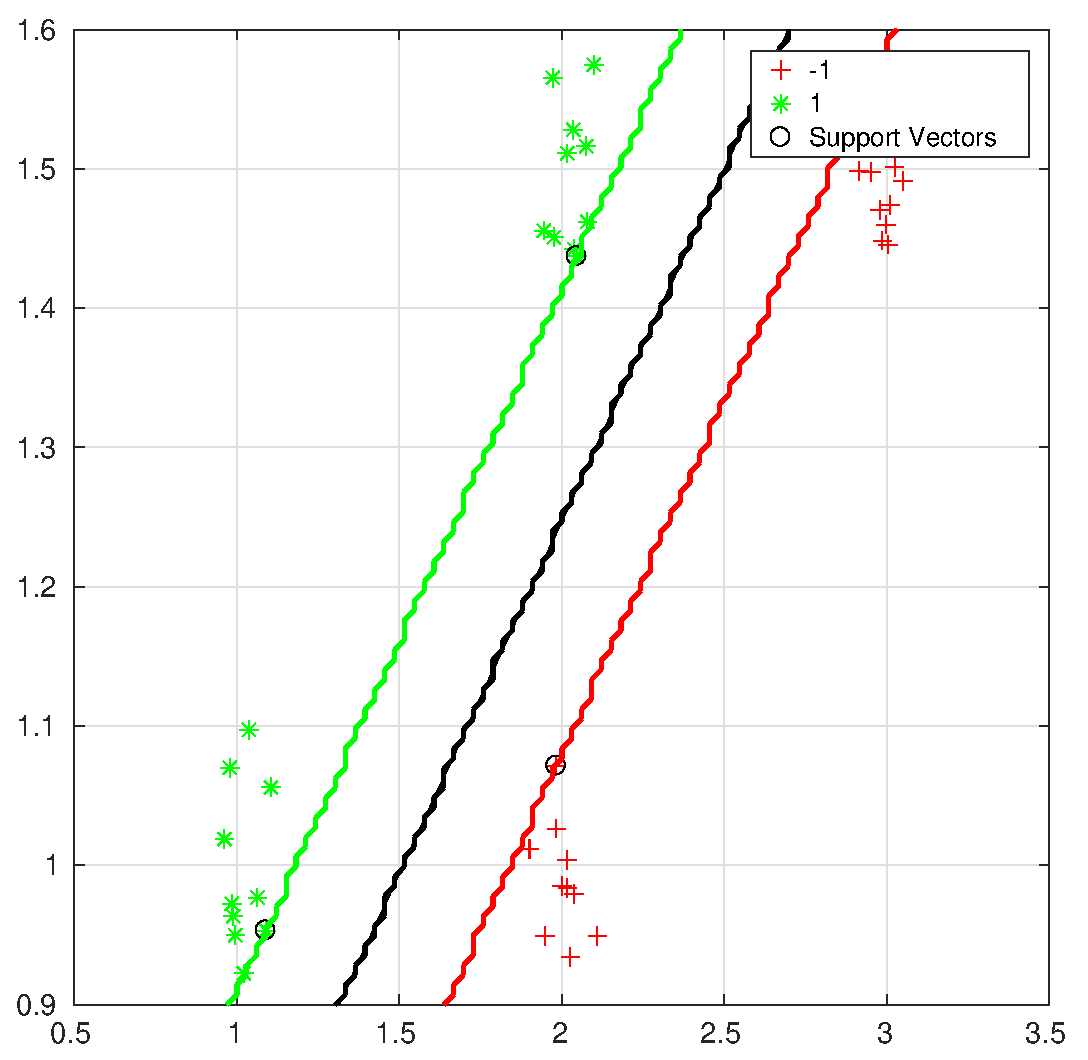
\includegraphics[width=0.36\textwidth]{SolutionMaterial/svm_sigma_5.eps}}
 	\subfigure[\label{fig:svm_sigma_100}]{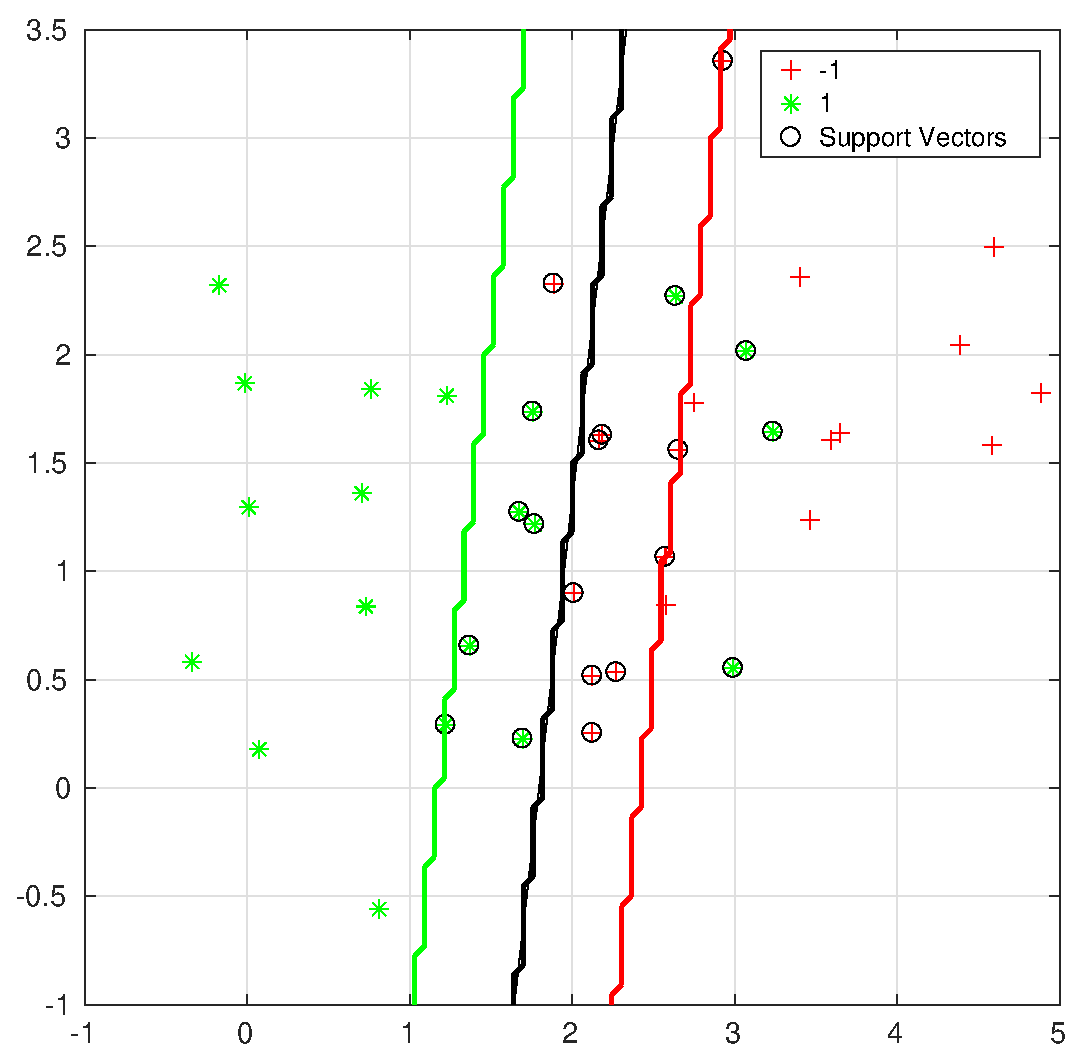
\includegraphics[width=0.36\textwidth]{SolutionMaterial/svm_sigma_100.eps}}
 	\subfigure[\label{fig:svm_sigma_140}]{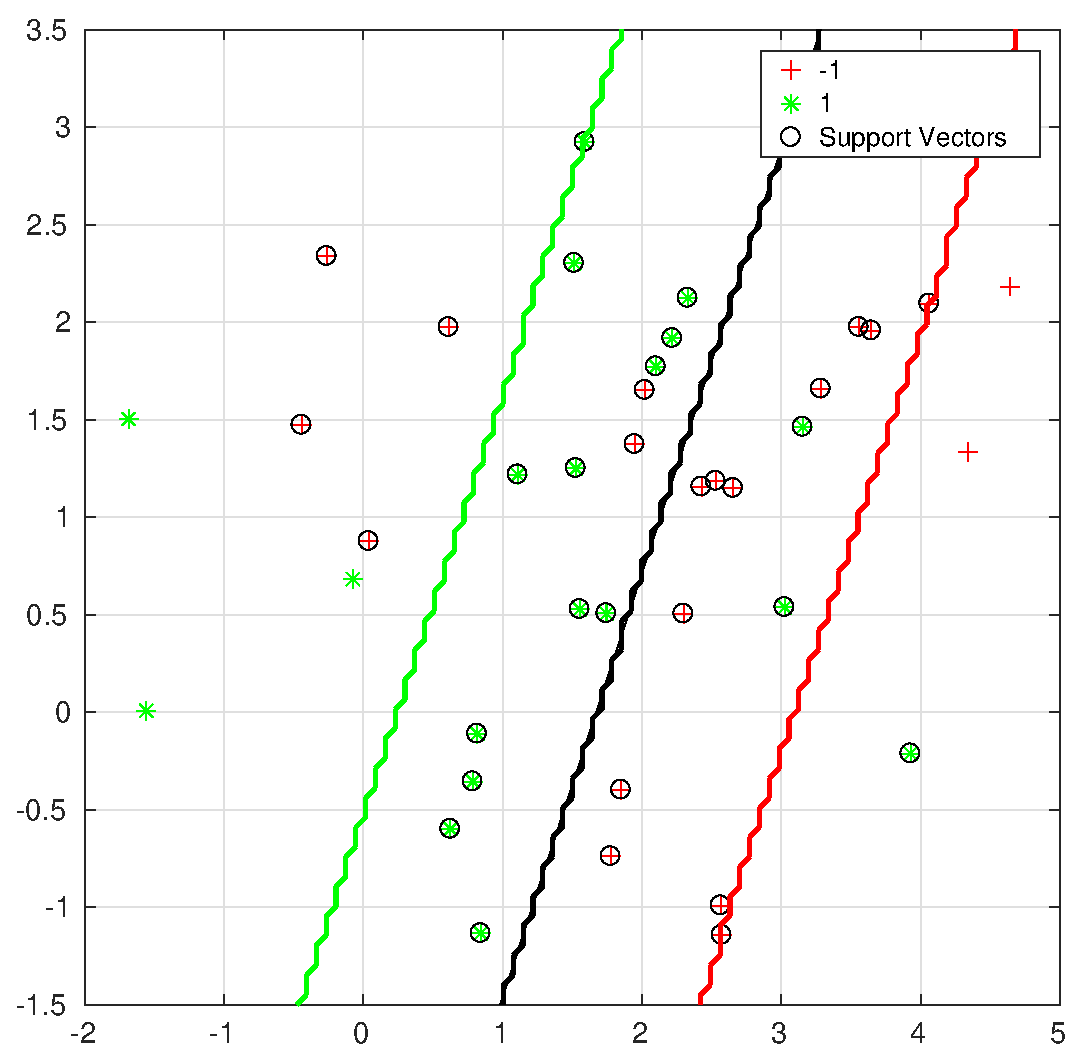
\includegraphics[width=0.36\textwidth]{SolutionMaterial/svm_sigma_140.eps}}
         \caption{Output of \emph{svmtrain} with different values of $\sigma$. (a), $\sigma = 0.05$. (b), $\sigma = 1$. (c), $\sigma = 1.4$.}
 \end{center}
\end{figure}

For $\sigma = 0.05$ on Fig.~\ref{fig:svm_sigma_5}, the samples of each classification group are close together creating clusters, hence 
there are no red markers on the upper left area or green markers on the lower right region, there are not even markers inside the 
margin area. The transversal length of the margin area is  $l_{m} = 0.29$ units.

On  Fig.~\ref{fig:svm_sigma_100} where  $\sigma = 1$, we can see that the two group of data is spread wider and they share a common 
area, which the support vector machine algorithm marks as the margin region. This time, there are some green markers on the lower right 
region and some red markers on the upper left region. This time the transversal length of the margin area is $l_{m} = 1.16$ units.

Finally, for $\sigma = 1.4$ the data is mixed together and the support vector machine algorithm\footnote{The value $\sigma = 1.4$ was critical, for slightly bigger values, the algorithm could not converge}  requires more support vectors, see Fig.~\ref{fig:svm_sigma_140}. The transversal length of the margin area is $l_{m} = 2.64$ units.

\subsection{Estimating Structural Risk}
\label{sec:ExperimentEstimatingStructuralRisk}

The two requested plots are presented on Fig.~\ref{fig:RisksVSValueC}, and Fig.~\ref{fig:RiskVSNElements}. The purpose
of these two graphs was to corroborate that as the empirical risk reduces as the value of $C$ tends to infinity, the actual and structural risks
increase, while the actual risk bounds both the empirical and estructural risk.

\begin{figure}[ht!]
 \begin{center}
  	\subfigure[\label{fig:RisksVSValueC}]{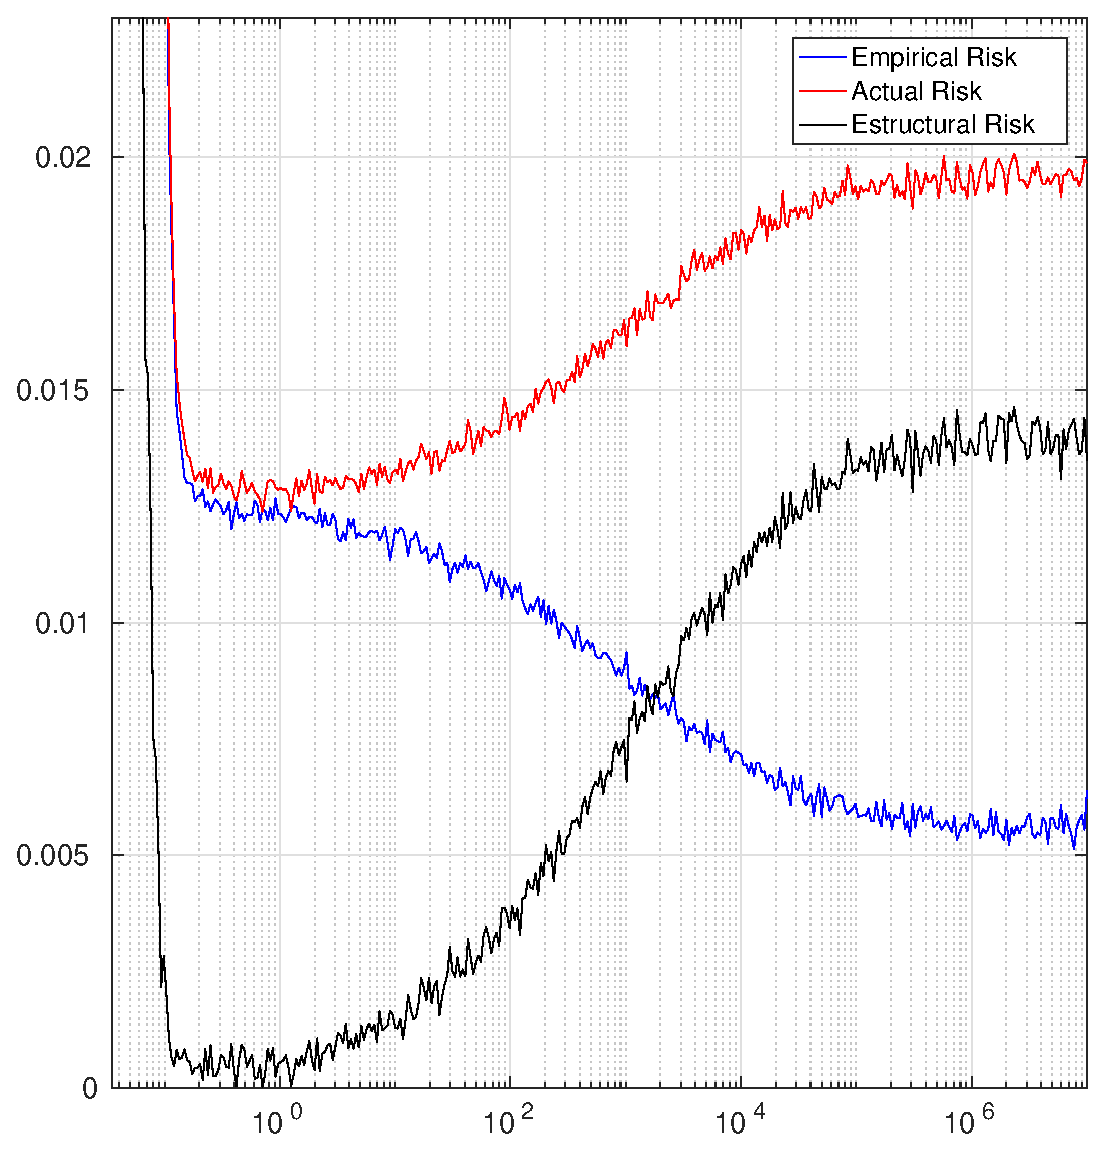
\includegraphics[width=0.40\textwidth]{SolutionMaterial/RisksVSValueC2.eps}}
 	\subfigure[\label{fig:RiskVSNElements}]{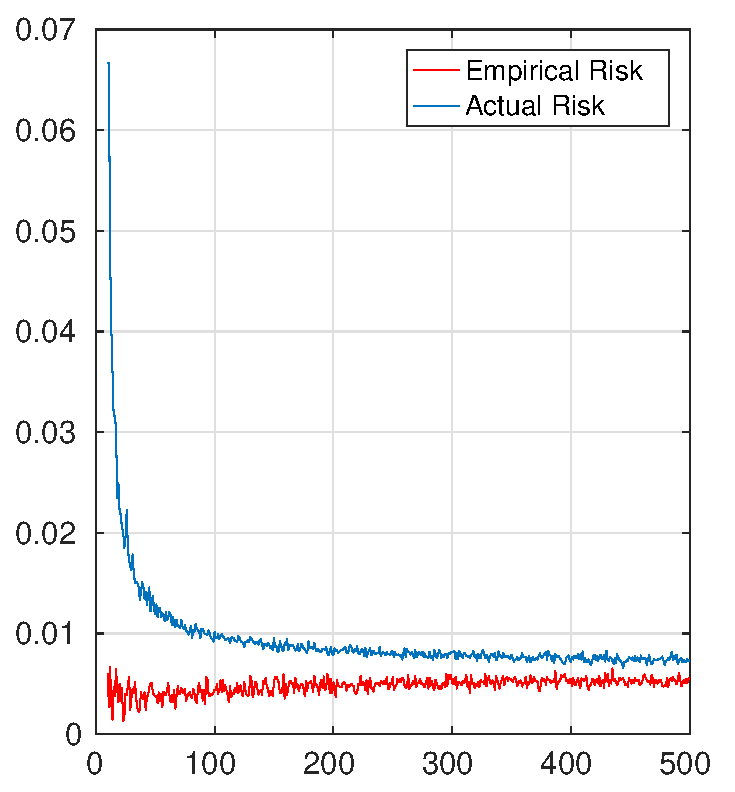
\includegraphics[width=0.40\textwidth]{SolutionMaterial/RiskVSNElements.eps}}
         \caption{Evolution of empirical and actual risk with respect to (a), value $C$. (b), the number of predictors $N$.}
 \end{center}
\end{figure}

The file \verb|data.m| was used to generate both the training and test data. A key element to obtain the results described earlier on is to
compute several executions and then average them, that is, we conducted $1000$ realizations; additionally, the choice of the interval for the free parameter $C$ is instrumental, the interval of $C$ is $[10^{-2},10^{7}]$.


\subsection{SVM for Regression}
\label{sec:ExperimentSVMRegression}

\begin{figure}[ht!]
 \begin{center}
  	\subfigure[\label{fig:SimulatedProccess}]{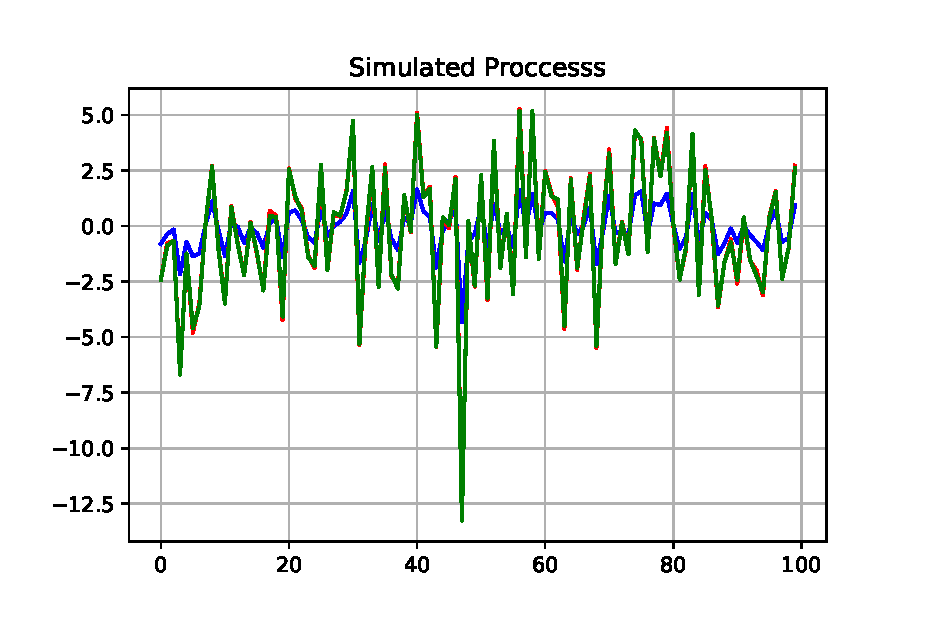
\includegraphics[width=0.56\textwidth]{SolutionMaterial/SimulatedProccess.eps}}
 	\subfigure[\label{fig:rmserror}]{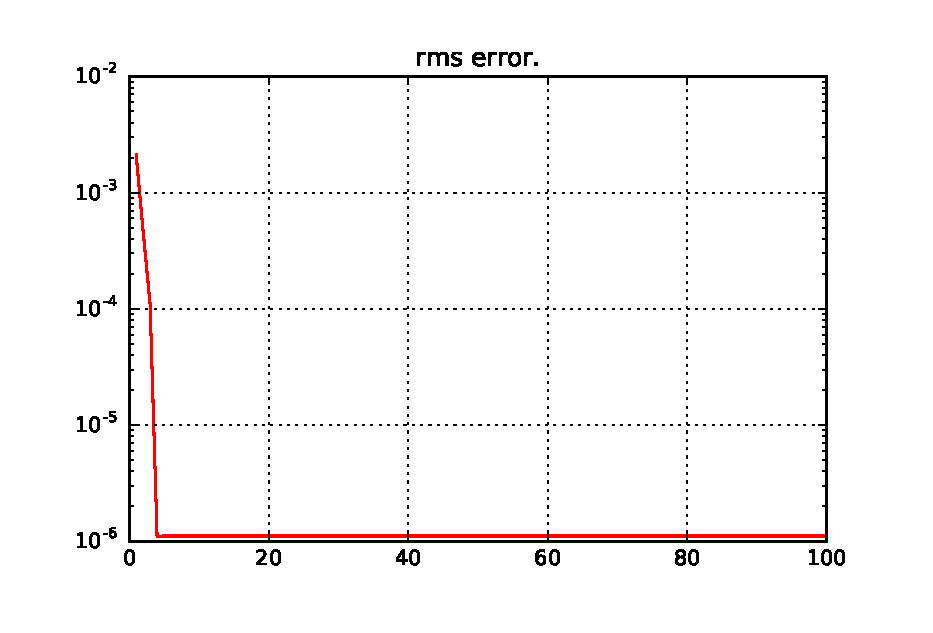
\includegraphics[width=0.56\textwidth]{SolutionMaterial/rms_error.eps}}
         \caption{SVM for regression (a), Simulated process: the blue represents the input $x[n]$, the red line is the evolution of the process $y[n]$, and 
         the green line is $o[n]$. (b), RMS Error.}
 \end{center}
\end{figure}
%%%%%%%%%%%%%%%%%%%%%%%%%%%%%%%%%%%%%%%%%%%%%%%%%%%%%%%%%%%%%%%%%%%%%%%%%%%%%%%%

\section{Conclusion}
\label{sec:conclusion}

\subsection{Construction of a classifier with the model parameters}
\label{sec:ConclusionsConstructionClassifierModelParameters}

The key differences are: the constructed machine is not conducting a regularization

\subsection{Graphical representation of an SVM}
\label{sec:ConclusionsGraphicalRepresentationSVM}
    
the support vector machine algorithm performs well for  Fig.~\ref{fig:svm_sigma_5}. it does not have problems
at classifying because the data is already clustered according to its label.

For  Fig.~\ref{fig:svm_sigma_100}, the support vector machine include more samples as support vectors and  on Fig.~\ref{fig:svm_sigma_140} even more.

As the variance is bigger, the support vector machine algorithm is pushed harder.

 \subsection{Estimating Structural Risk}
 \label{sec:ConclusionEstimatingStructuralRisk}

We want to know the actual risk of a trained machine because we want to know how susceptible our trained machine is under a new
subset of data. However, the definition given on \cite{Burges1998} requires knowledge of the probability function associated with the
data, which is not available. Hence, we need to estimate this quantity. We do that by generating a new data set and use it as our test set, 
and then use Equation \ref{eq:Error} with the test set.

We think the reason behind of why the minimum actual risk does not coincide with the intersection of the other two errors has to do with 
complexity. Note that on Figure.~\ref{fig:RisksVSValueC} the minimum of the actual risk is almost the same as the value of the empirical risk 
for low values of $C$. This is because the trained machine has a low value $C$ so the machine has the same clearance in both the train and test 
set. However, as $C$ increases, the complexity does too, so the trained machined is forced to map better the training data to the training labels, 
but at the same time the machine is not going to perform as well with a new set of data as the test set. Then the actual error is going to increase.
The minimum of the actual risk is not going to coincide with the intersection of the other two errors because the manipulation of the value $C$ is
a trade off between the complexity and regularization: The minimum of the actual error is one side of the coin; the machine does not overfit but it
is too simple. The intersection happens in the middle of the logarithmic domain, where $C$ is bigger and you have made your machine more complex 
so it can describe the data closer. 
 
 For the second question, the procedure seems consistent, we have more data, but after $N \approx 70$ you don't gain more.
 
% \subsection{SVM for Regression}
%\label{sec:ConclusionSVMRegression}


%%%%%%%%%%%%%%%%%%%%%%%%%%%%%%%%%%%%%%%%%%%%%%%%%%%%%%%%%%%%%%%%%%%%%%%%%%%%%%%%

%References are important to the reader; therefore, each citation must be complete and correct. If at all possible, references should be commonly available publications.


%\pagebreak

\bibliographystyle{IEEEtran}
\bibliography{References}

%%%%%% APPENDIX %%%%%%%
%q\input{Appendix}
\end{document}
